\chapter{Literature Review}

\section{Multi-Agentic Systems}

 Multi-agent LLMs has become a popular topic \cite{guo2024largelanguagemodelbased}. A large proportion of works focus on social simulation \cite{park2023generativeagentsinteractivesimulacra} and frameworks \cite{li2023camelcommunicativeagentsmind}. Based on the success of them, some
 works explore the game settings \cite{light2023avalonbenchevaluatingllmsplaying}, world wars \cite{hua2024warpeacewaragentlarge}, economy markets \cite{li2024econagentlargelanguagemodelempowered}, recommendation systems\cite{zhang2024generativeagentsrecommendation}, and pandemics \cite{Ghaffarzadegan_2024}. Others advance problem solving, focusing on reasoning of short text via multi-agent debating and discussing for different tasks in reasoning \cite{du2023improving, Xiong_2023, tang2024medagentslargelanguagemodels}, mechanics problems, paper review, knowledge graph construction \cite{ye2024isolationmultiagentsynergyimproving}, and code intelligence.

\subsection{Long Context Modeling for LLMs} 

Numerous application scenarios demand extremely long contexts, such as question answering, document and dialogue summarization, and code completion, where the inputs contain entire books and long articles. To tackle the challenge with long context tasks, two major directions have been explored as shown in (Table \ref{tab:prompting-strategies}): input reduction and window extension. \textit{Input reduction} reduces the length of the input context before feeding to downstream LLMs. Truncation approaches directly truncate the input. Retrieval Augmented Generation (RAG)  \cite{xu2024retrievalmeetslongcontext} extends this direction by retrieving the most relevant chunks through embedding similarity. However, because of low retrieval accuracy, LLMs could receive an incomplete context for solving the task, hurting performance \cite{yan2024correctiveretrievalaugmentedgeneration}. \textit{Window extension} extends the context window of LLMs via finetuning to consume the whole input. For instance, the context window increases from 1024 (GPT-2), 2048 (GPT-3), to 128k (GPT-4) \cite{openai2024gpt4technicalreport, Radford2019LanguageMA}. Moreover, the newest version of Claude-3 \cite{claude} supports 200k context windows. However, when the window becomes longer, LLMs struggle to focus on the needed information to solve the task, suffering from ineffective context utilization such as the “lost in the middle” issue \cite{liu2023lostmiddlelanguagemodels}. Recently, a few studies have employed text chunking algorithms to divide and process lengthy text inputs.
 
\subsection{Complex Task Reasoning} 
Previous works on complex reasoning have focused on decomposing the complex question into sub-questions to solve them step-by-step \cite{perez2020unsupervisedquestiondecompositionquestion}. Decomposed Prompting \cite{khot2023decomposedpromptingmodularapproach} leverages some predefined modules to classify each decomposed sub-question, then further decompose if needed. Recently, methods such as Chain-of-Thought \cite{wei2023chainofthoughtpromptingelicitsreasoning}, Least-to-Most prompting \cite{zhou2023leasttomostpromptingenablescomplex} and Pearl \cite{sun2023pearlpromptinglargelanguage} have been proposed for LLMs. 

\begin{table}[h!]
    \centering
    \resizebox{\textwidth}{!}{%
    \begin{tabular}{@{}llccccccc@{}}
        \toprule
        \textbf{Category}       & \textbf{Example Work}   & \textbf{Rec.} & \textbf{Foc.} & \textbf{No Train} & \textbf{Read} & \textbf{Agent}  & \textbf{Applicability} & \textbf{Inter.} \\ 
        \midrule
        Input Reduction         & Truncation & \xmark       & \cmark        & \cmark            & $k$           & Single          & Generic               & Low             \\
                                & RAG       & \xmark       & \cmark        & \xmark            & $n + k$       & Single          & Query-based          & Medium          \\
        \midrule
        Window Extension        & Position Interpolation  & \cmark & \xmark & \xmark & $n$ & Single & Generic & Low \\
                                & Long Context          & \cmark & \xmark & \xmark & $n$ & Single & Generic & Low \\
        \midrule
        Multi-agent LLMs        & Chain-of-Agents     & \cmark       & \cmark        & \cmark            & $n$           & Multiple        & Generic               & High            \\
        \bottomrule
    \end{tabular}
    }
    \caption{Comparison between Chain-of-Agents and prior methods for long-context tasks. Rec./Foc.:
 being able to mitigate inaccurate receptive field/long context focusing issues. Read: the number of
 tokens as model input, where n is the total input length, k is the context window limit of LLMs.
 Inter.: the interpretability of the approach. Note that RAG is ‘medium interpretable’ because of the
 re-ranked chunks.}
    \label{tab:prompting-strategies}
\end{table}

\section{Code Completion Systems}

Large Language Models (LLMs) have demonstrated impressive capabilities in code completion tasks \cite{codeium, marscode, copilot}, where they assist developers by predicting and generating new code in real-time. Much of existing research focus on leveraging repository-level contextual information to provide opportunities to improve code completion. This context includes core function definitions, configuration files, and code snippets from elsewhere in the repository that align with the developer’s current logic (Figure \ref{fig:completion}). Beyond context, a series of algorithms select relevant code snippets or comments from the current file and other sources before being filtered and assembled into the final prompt \cite{copilotx}. By incorporating these strategies, LLMs can generate more accurate and context-aware code, ultimately increasing the acceptance rate of suggestions and further enhancing coding efficiency. 

\begin{figure}
    \centering
    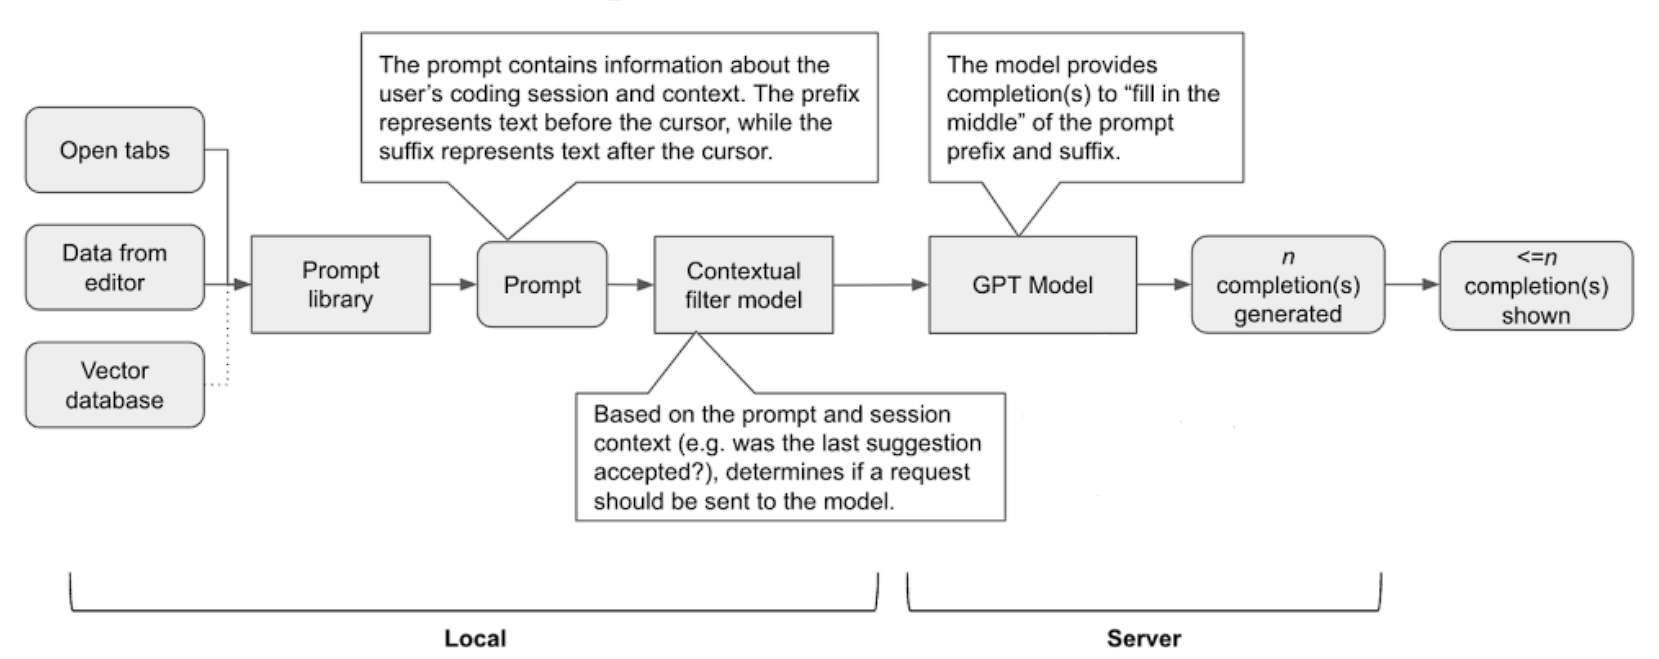
\includegraphics[width=0.8\linewidth]{fig/completion.png}
    \caption{Life of a Completion}
    \label{fig:completion}
\end{figure}

\subsection{Associated Challenges}

Several challenges remain when deploying these models in real-world environments.

\subsubsection{Limited Contextual Understanding}
While relying on the content of the file the user is working on can generate useful suggestions \cite{copilotx}, it often lacks the broader repository-level context that can be crucial for more complex tasks \cite{banerjee2024contextmatterspushingboundaries}. For instance, relevant function definitions, configuration files, or similar snippets elsewhere in the repository may not be considered, limiting the model’s ability to generate the most accurate or context-aware code.

\subsubsection{User Behavior and Intent Recognition}
Developers frequently browse and edit code across multiple files while working on a particular task. This cross-file behavior contains implicit information about the developer’s intent \cite{coeditor, coedpilot} that can be valuable for code generation. However, current code completion systems \cite{copilot, codeium, marscode} do not effectively incorporate this user behavior, resulting in suggestions that may not fully align with the developer’s immediate goals. 

\subsubsection{Efficient Retrieval of Information}
Retrieving necessary contextual information can be time-consuming and computationally expensive. For example, developers working on a large project may need relevant snippets, function signatures, or symbol definitions from different parts of the repository to guide their current task. However, real-world deployment of LLM tools introduces strict latency requirements, especially in code completion, where developers expect suggestions to appear instantly \cite{cursorai}. The challenge is to balance accuracy while keeping response times within acceptable limits.


\subsection{Methods for Better Contextual Information}

To address these challenges, recent research have integrated machine learning with dependency-aware planning to address the complexities of multi-file editing in large projects.

\subsubsection{Context-Aware Edit Representation}

Using prompting techniques and various encoding schemas, the prompt captures both the content of each edit and its surrounding context, enabling precise and contextually relevant suggestions. By leveraging Fill-in-the-Middle (FiM) \cite{bavarian2022efficienttraininglanguagemodels}, the model predicts not only the immediate next steps but also intermediate edits, thus improving its adaptability to non-linear workflows. Similarly, line-diff encoding emphasizes the differences between code versions, allowing the framework to focus on incremental changes and better understand the developer's intent.

\subsubsection{Dependency-Aware Planning}

Dependency-aware planning systems complement the process by tracking both syntactic and semantic relationships within the codebase \cite{coedpilot}. By incrementally updating dependency graphs with each edit, these systems ensure adaptive, repository-wide consistency and effectively anticipate the downstream impacts of code changes. 

\subsubsection{Interactive and Multi-Round Editing}

Human-in-the-loop frameworks (Figure \ref{fig:trae}) make code completion more intuitive by incorporating user inputs and feedback into the editing process. These frameworks dynamically adapt to prior changes, leveraging a multi-stage analysis to identify the files and lines most likely to require updates. This approach allows developers to guide the model's recommendations, ensuring that subsequent edits are contextually relevant and aligned with user intent. By fostering an interactive and collaborative editing experience, human-in-the-loop frameworks \cite{marscode, copilot, cursorai} simplify complex code completion tasks and enhance overall developer productivity.

\subsubsection{Heuristic-Based Approaches}

By applying rule-based strategies that streamline dependency management and refine edit locations, these approaches prioritize changes in files or functions closely related, syntactically or functionally, to the original edit, reducing redundant processing. Common heuristics \cite{coeditor, coedpilot} include proximity-based prioritization, which applies edits within syntactically related areas, and "hotspot" detection, focusing on frequently modified sections of code. By integrating these heuristics, systems can more efficiently direct computational resources to areas with higher propagation likelihood. This combination allows heuristic methods to handle both predictable, pattern-based changes and complex, adaptive editing scenarios.

\vspace{1cm}

\begin{figure}
    \centering
    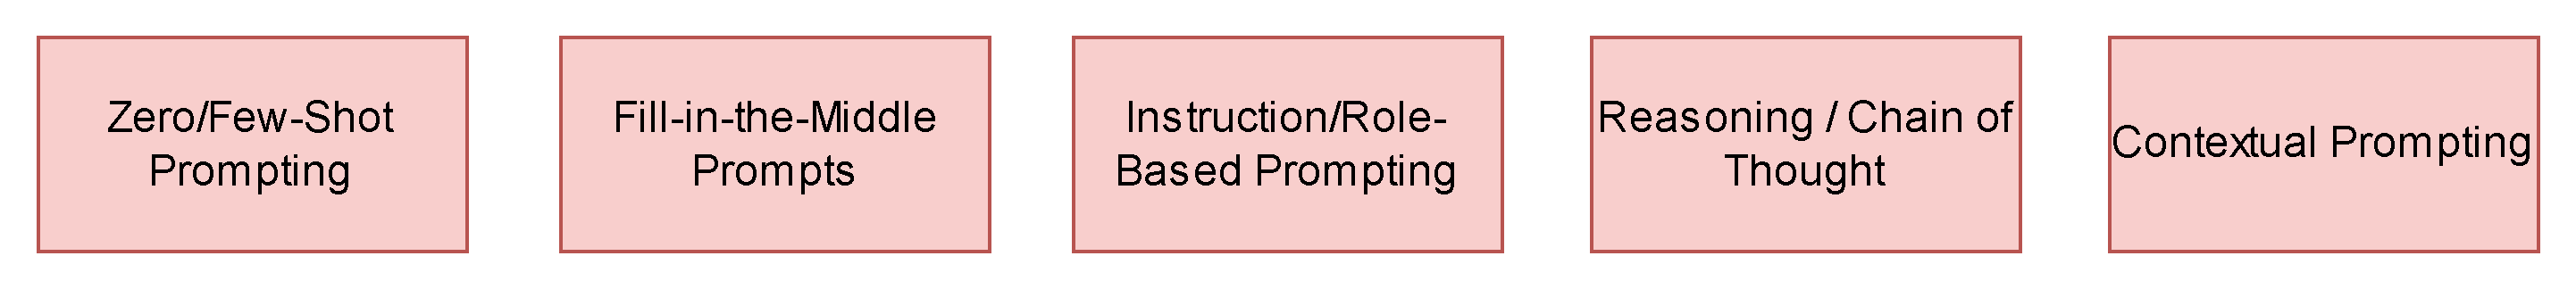
\includegraphics[width=0.8\linewidth]{fig/prompt_strats.png}
    \caption{Various prominent prompting strategies}
    \label{fig:prompt}
\end{figure}

\begin{figure}[h]
    \centering
    % First Image
    \begin{minipage}[t]{0.8\textwidth}
        \centering
        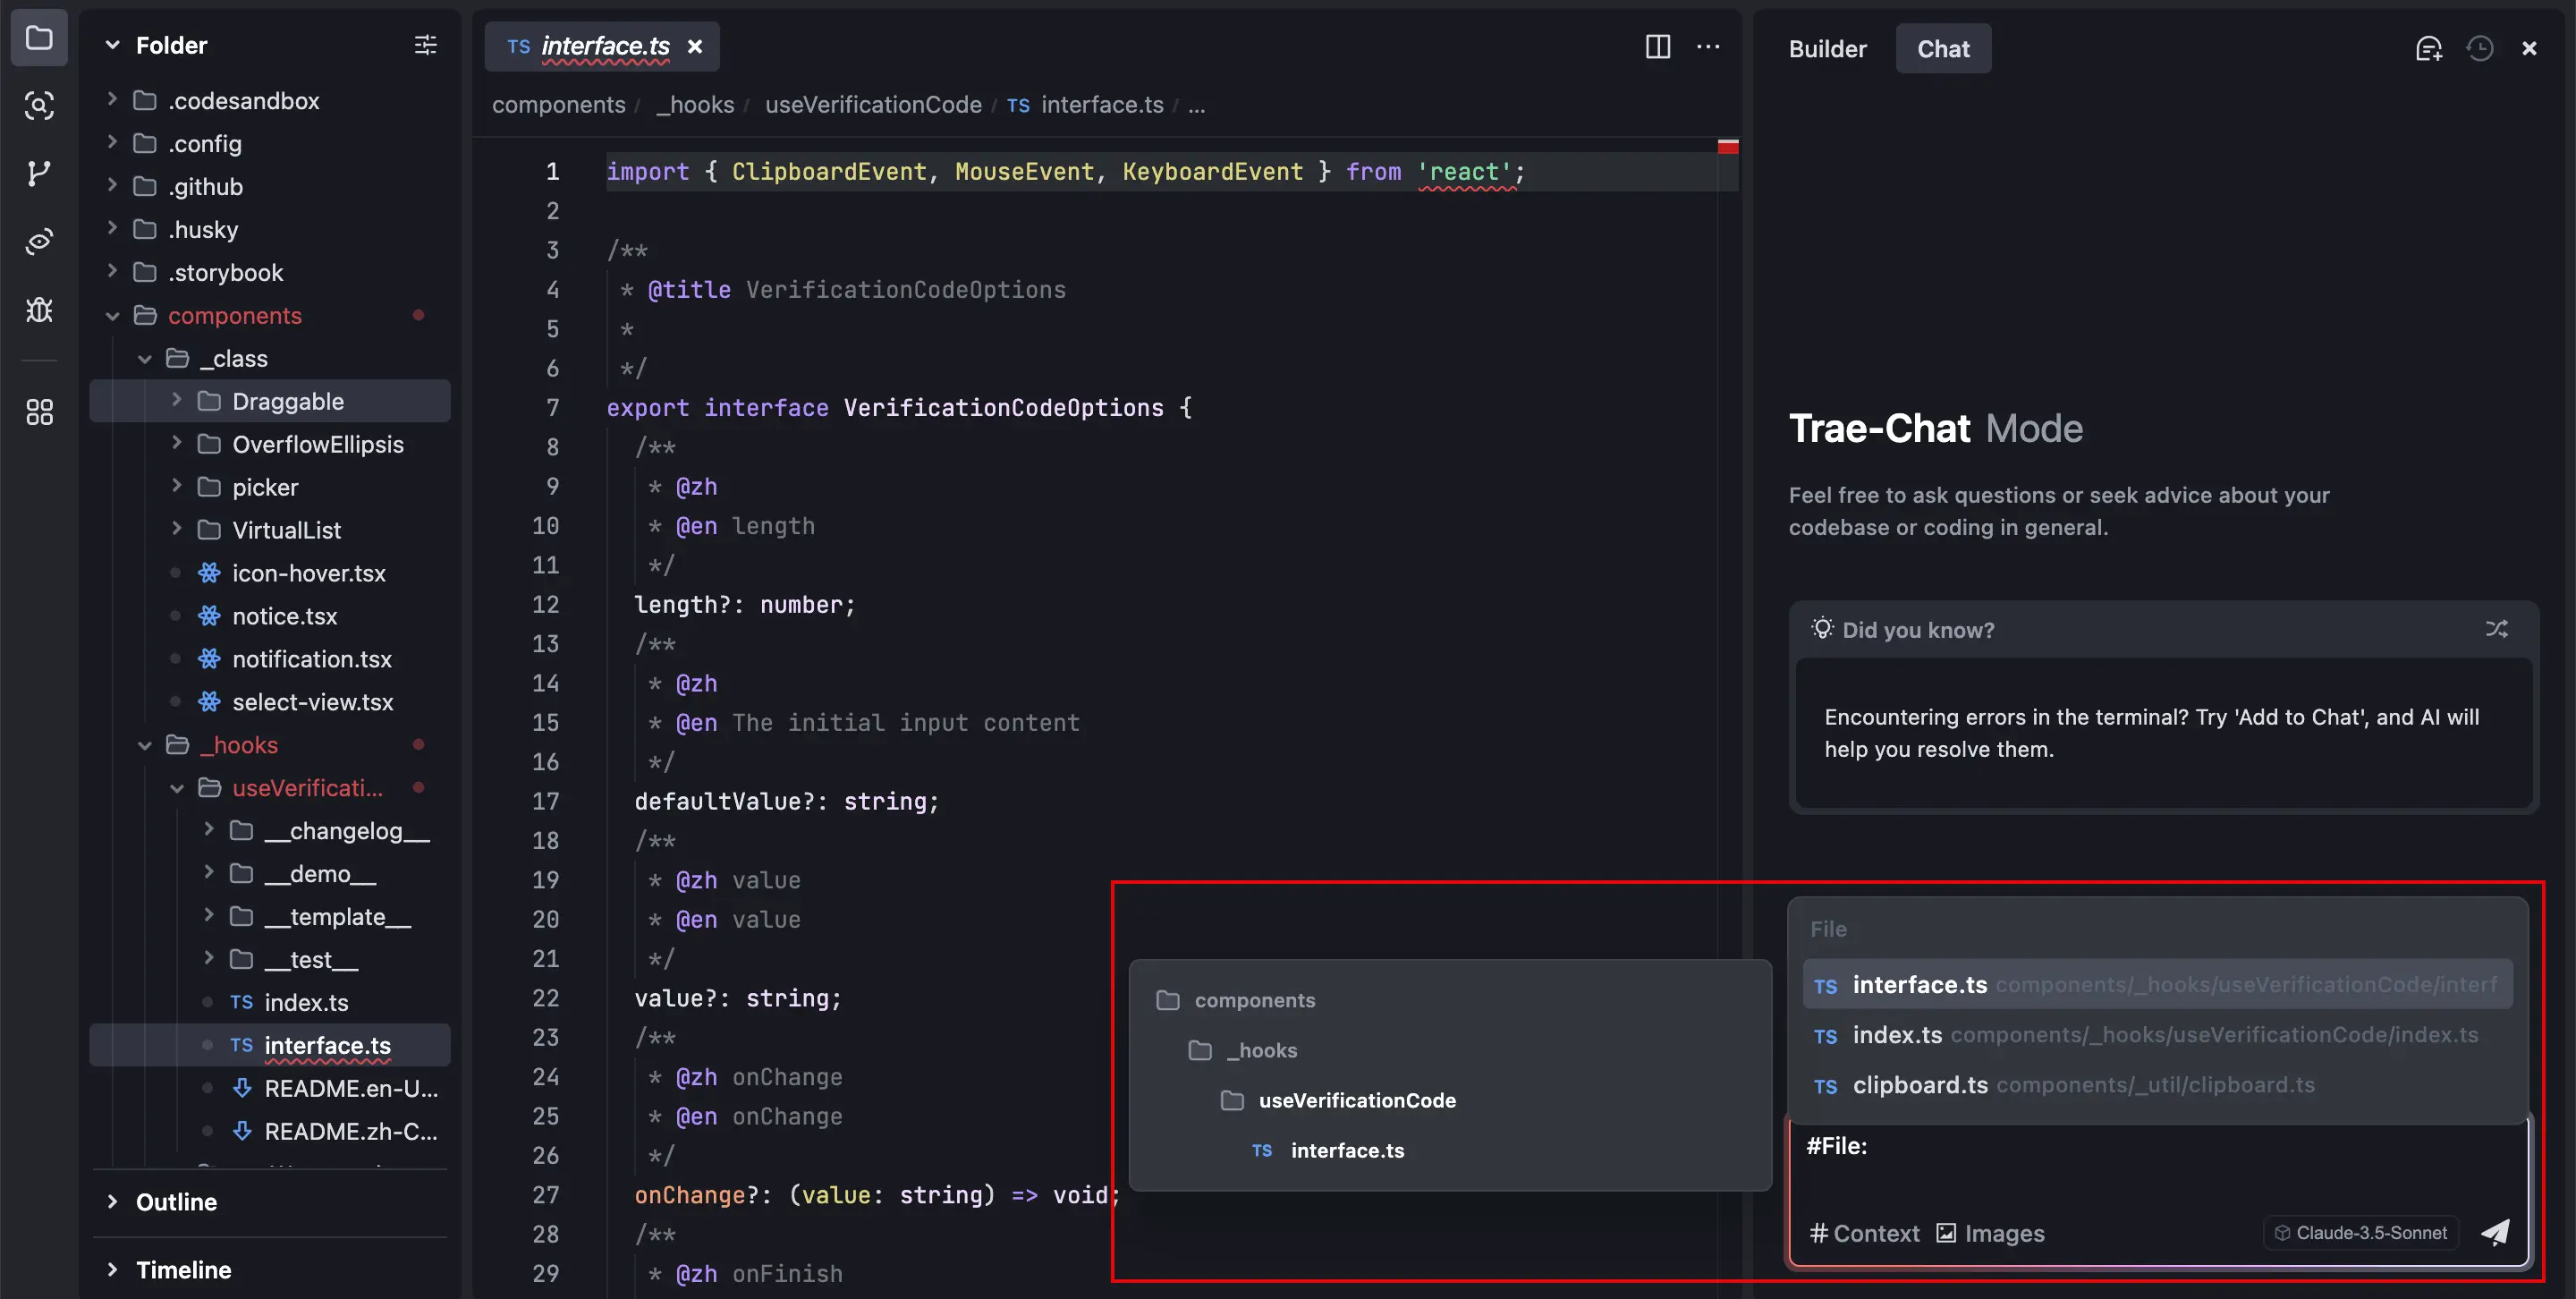
\includegraphics[width=1\linewidth]{fig/trae-1.png} % Replace with your image file
        \caption*{(a) Select relevant files as context for multi-file edits.} % Caption without label
        \vspace{0.5cm}
    \end{minipage}
    \begin{minipage}[t]{0.8\textwidth}
        \centering
        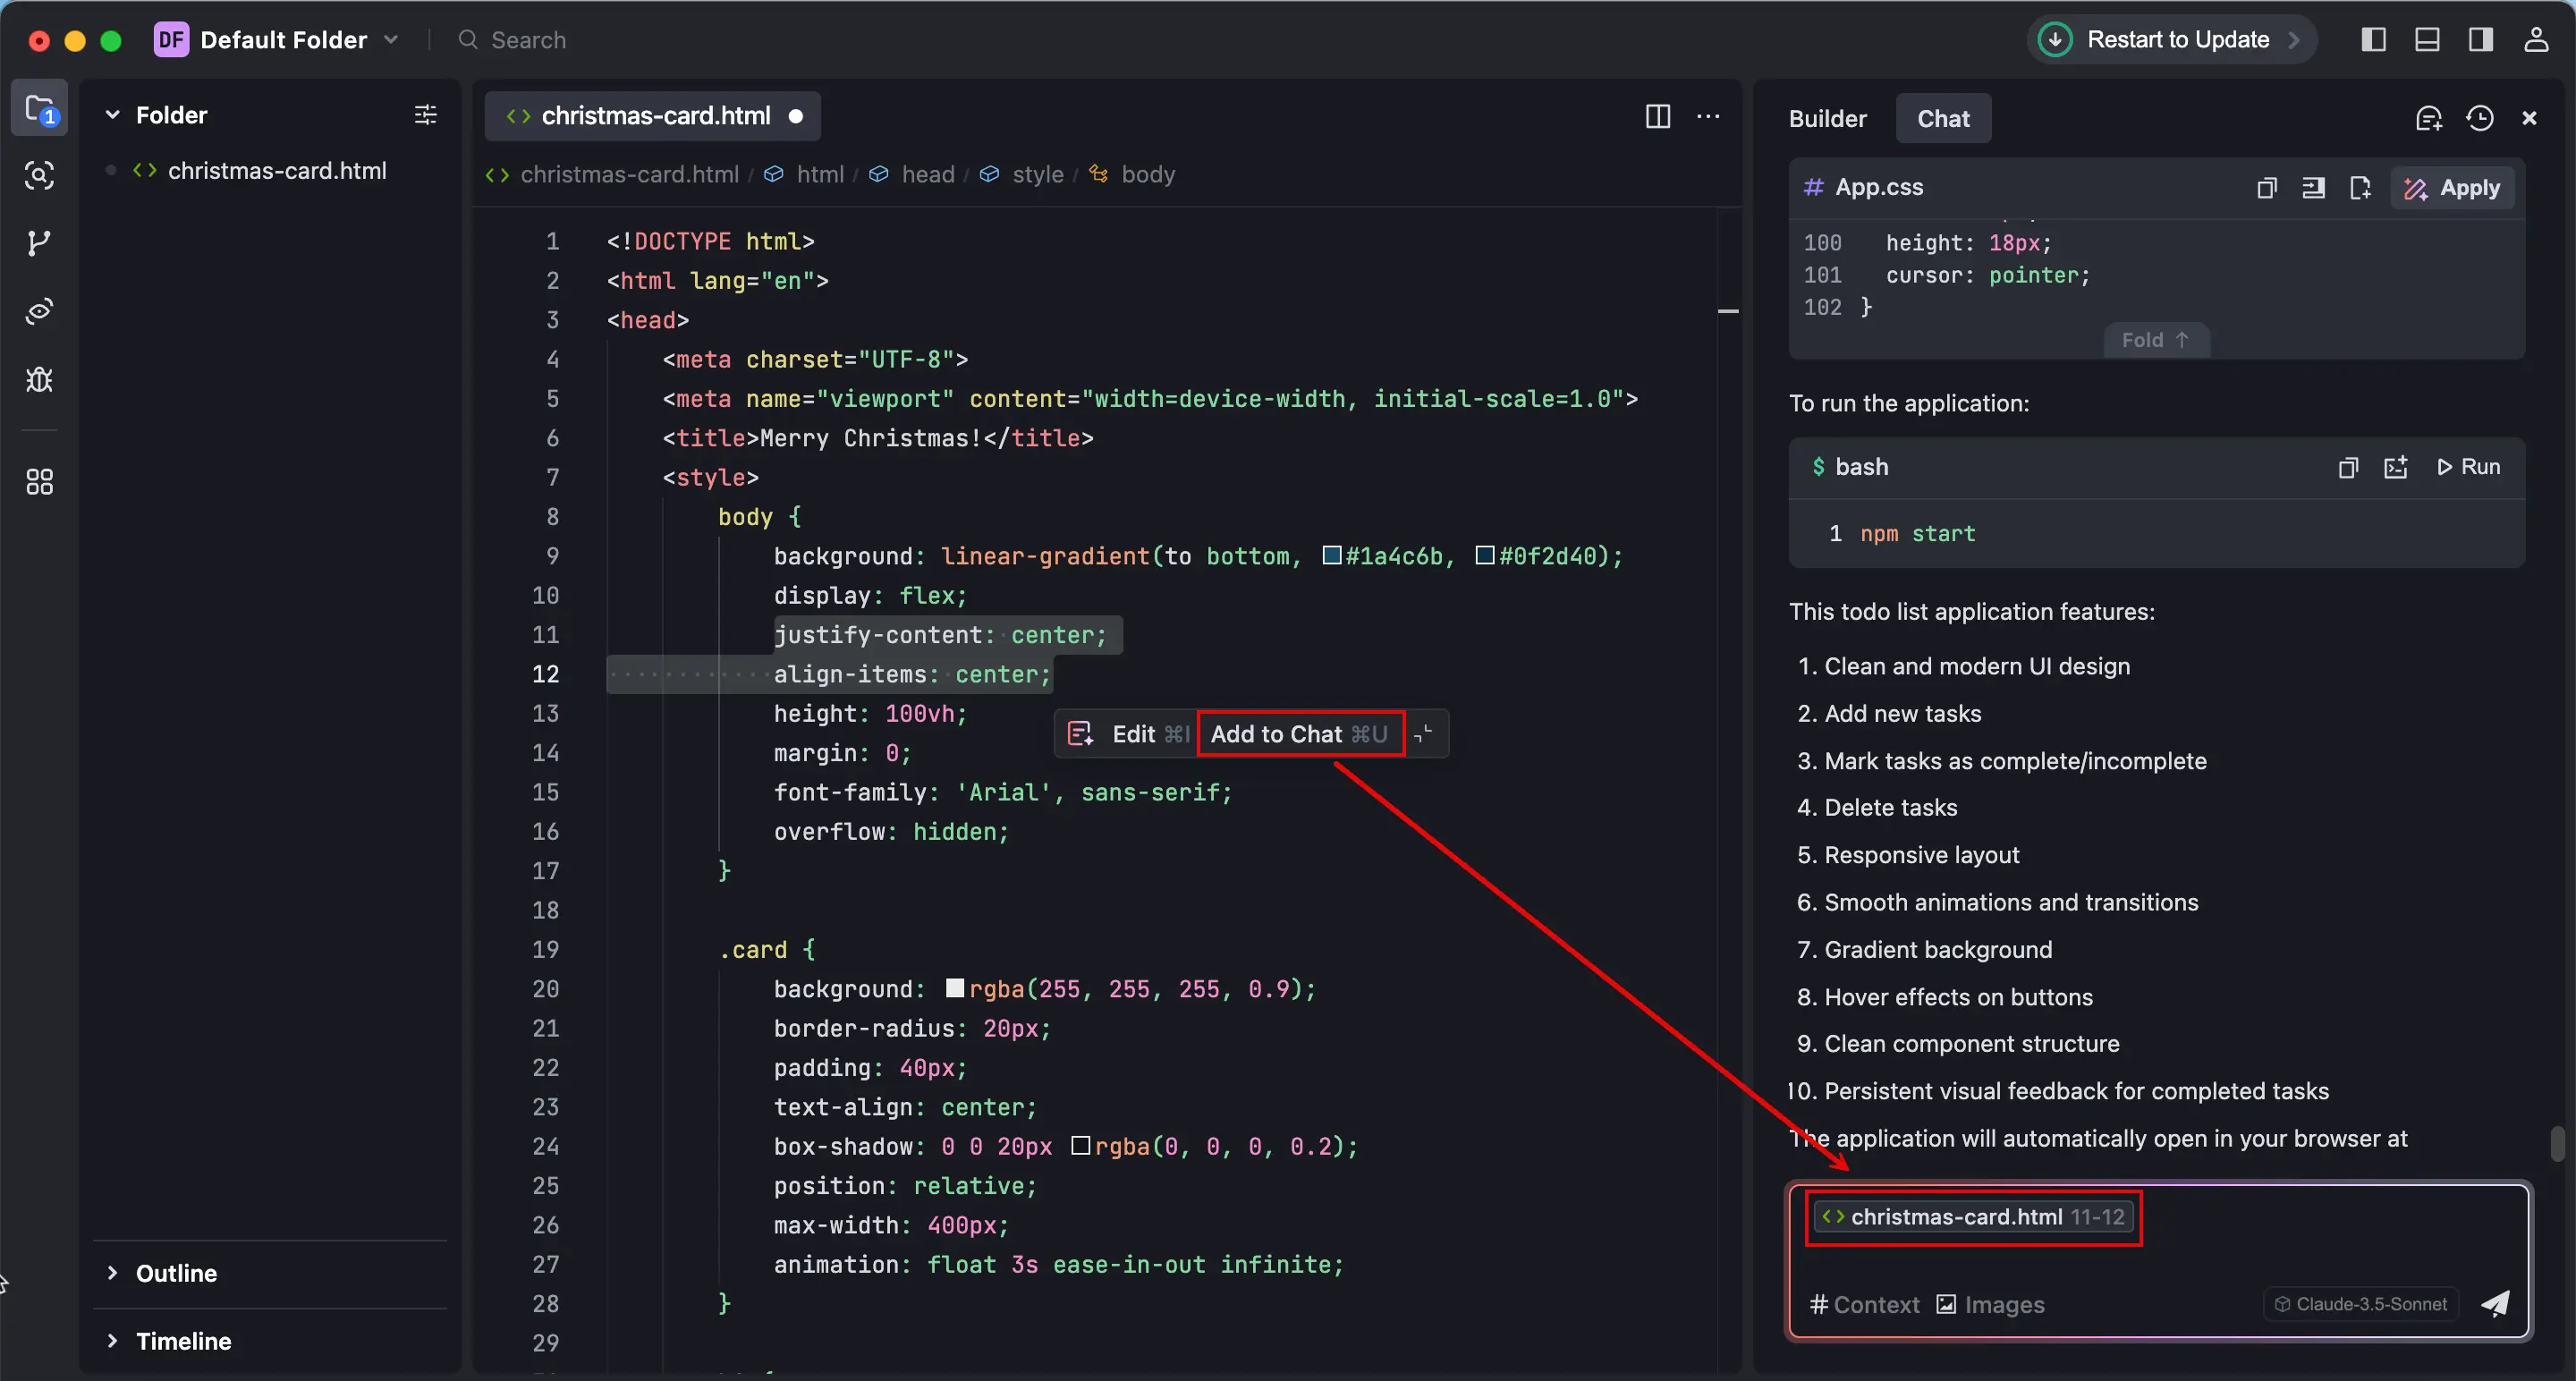
\includegraphics[width=1\linewidth]{fig/trae-2.png} % Replace with your image file
        \caption*{(b) Option to add inline code as context to chat bot.} % Caption without label
    \end{minipage}
    % Overall Caption
    \caption{Human-in-the-Loop Design in AI IDE, Trae AI.}
    \label{fig:trae}
\end{figure}

